\documentclass{article}
\usepackage{graphicx}
\usepackage{amsmath}
\usepackage[margin=3cm]{geometry}
\usepackage{listings}
\usepackage{xcolor}
\usepackage{hyperref}
\usepackage{listings}

\usepackage{graphicx}

\title{Data Modelling and Databases}
\date{2023-06-21T11:21:37+02:00}
\author{Gnkgo}

\begin{document}
\maketitle

\clearpage

\tableofcontents

\clearpage

\section{Normal Forms}

\subsection{First Normal Form}
\begin{enumerate}
    \item Using row order to convey information is not permitted
    \item Mixing data types within the same column is not permitted
    \item Having a table without a primary key is not permitted
    \item Repeating groups are not permitted
\end{enumerate}

\textbf{The Key}
\begin{itemize}
    \item Values in each column should not be tables
    \item Records in the table should be unique
    \item Primary key
\end{itemize}

\begin{figure}[h]
    \centering
    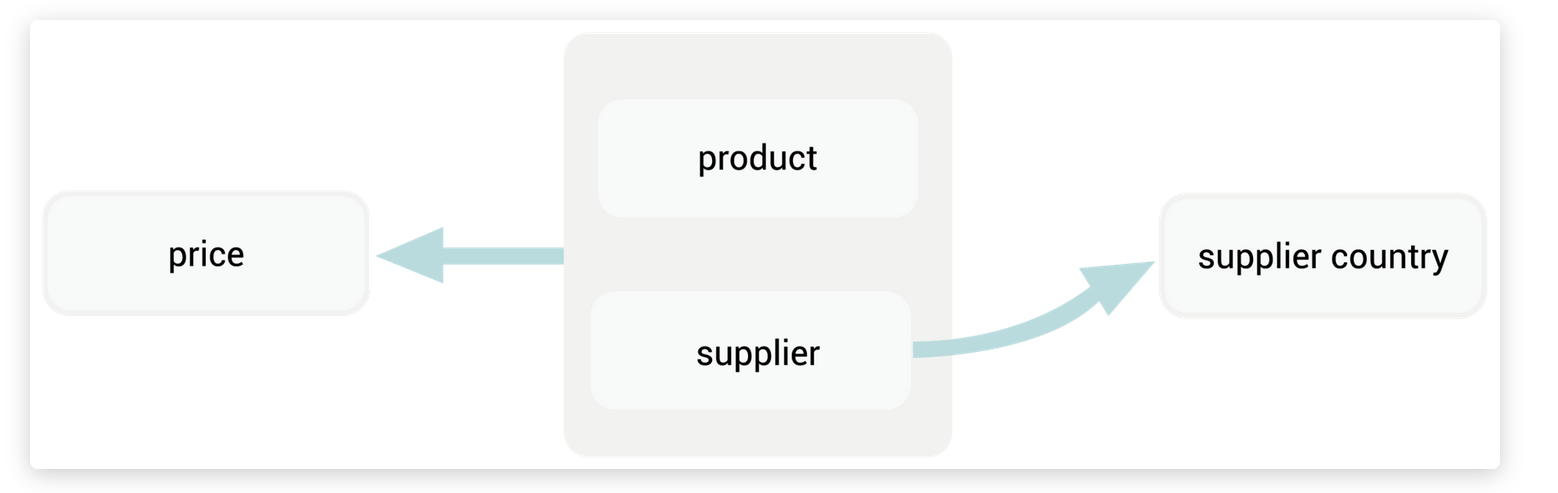
\includegraphics[width=0.5\textwidth]{assets/first_normal_form.png}
    \caption{First Normal Form}
\end{figure}
\textbf{Higher Form}
Find the dependencies and split them up
\begin{align*}
    AB & \rightarrow C \\
    B  & \rightarrow D
\end{align*}

We see that $AB$ is a superkey, but $B$ is a subset.

\begin{align*}
    R1 & = \{A, B, C\} \\
    R2 & = \{B, D\}
\end{align*}

Here's the general algorithm for normalizing a table from 1NF to 2NF.

Suppose you have a table $R$ with scheme $S$ which is in 1NF but not in 2NF.
Let $A \rightarrow B$ be a functional dependency that violates the rules for
2NF, and suppose that the sets $A$ and $B$ are distinct ($A \cap B =
    \emptyset$).

Let $C = S - (A \cup B)$. In other words:
\begin{itemize}
    \item $A$ = attributes on the left-hand side of the functional dependency.
    \item $B$ = attributes on the right-hand side of the functional dependency.
    \item $C$ = all other attributes.
\end{itemize}

We can split $R$ into two parts:
\begin{itemize}
    \item $R1$, with scheme $C \cup A$.
    \item $R2$, with scheme $A \cup B$.
\end{itemize}

The original relation can be recovered as the natural join of $R1$ and $R2$: $R
    = R1 \text{ NATURAL JOIN } R2$

\subsection{Second Normal Form}
\begin{itemize}
    \item Each non-key attribute in the table must be dependent on the entire primary
          key.
    \item If you have a strict subset of the key, it is not in 2NF.
    \item If everything on the right side is a key, then it is in 2NF.
\end{itemize}

\textbf{The Whole Key}
\begin{itemize}
    \item No partial dependencies on the candidate keys.
    \item Columns must be dependent on the whole key.
\end{itemize}

\begin{figure}[h]
    \centering
    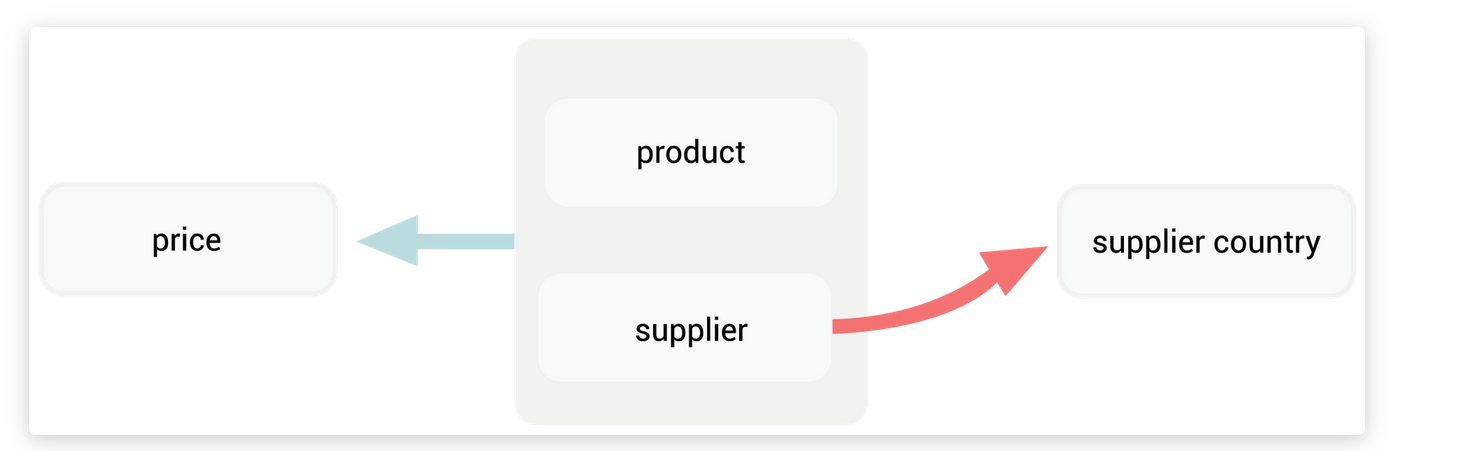
\includegraphics[width=0.5\textwidth]{assets/second_normal_form.png}
    \caption{Second Normal Form}
\end{figure}
\textbf{Higher Form - Synthesis Algorithm}
\begin{align*}
    R1 & = \{A, B, C, D, E, F\} \\
    A  & \rightarrow D          \\
    B  & \rightarrow C          \\
    B  & \rightarrow D          \\
    D  & \rightarrow E          \\
\end{align*}
ABF is a minimal key
Merge
\begin{align*}
    A & \rightarrow D \\ B &\rightarrow C, D \\ D &\rightarrow E \\
\end{align*}
Create a relation
\begin{align*}
    R1 & = \{A, D\}    \\
    R2 & = \{B, C, D\} \\
    R3 & = \{D, E\}    \\
\end{align*}
Does one of these relations contain a key of R? NO, so we add a relation with a
minimal key of R:
\begin{align*}
R4 &= \{A, B, F\}
\end{align*}
\subsection{Third Normal Form}
\begin{itemize}
    \item Each non-key attribute in the table must depend on the key, the whole key, and
          nothing but the key.
    \item If everything on the right side is a key, then it is in 3NF.
    \item No transitive relations.
    \item Left-hand side is either a super key or right-hand side is a prime attribute.
\end{itemize}

\textbf{Nothing but the Key (Attribute)}
\begin{itemize}
    \item Every non-key attribute is non-transitively (directly) dependent on the
          candidate key. The columns can only be dependent on the key columns.
\end{itemize}

\begin{figure}[h]
    \centering
    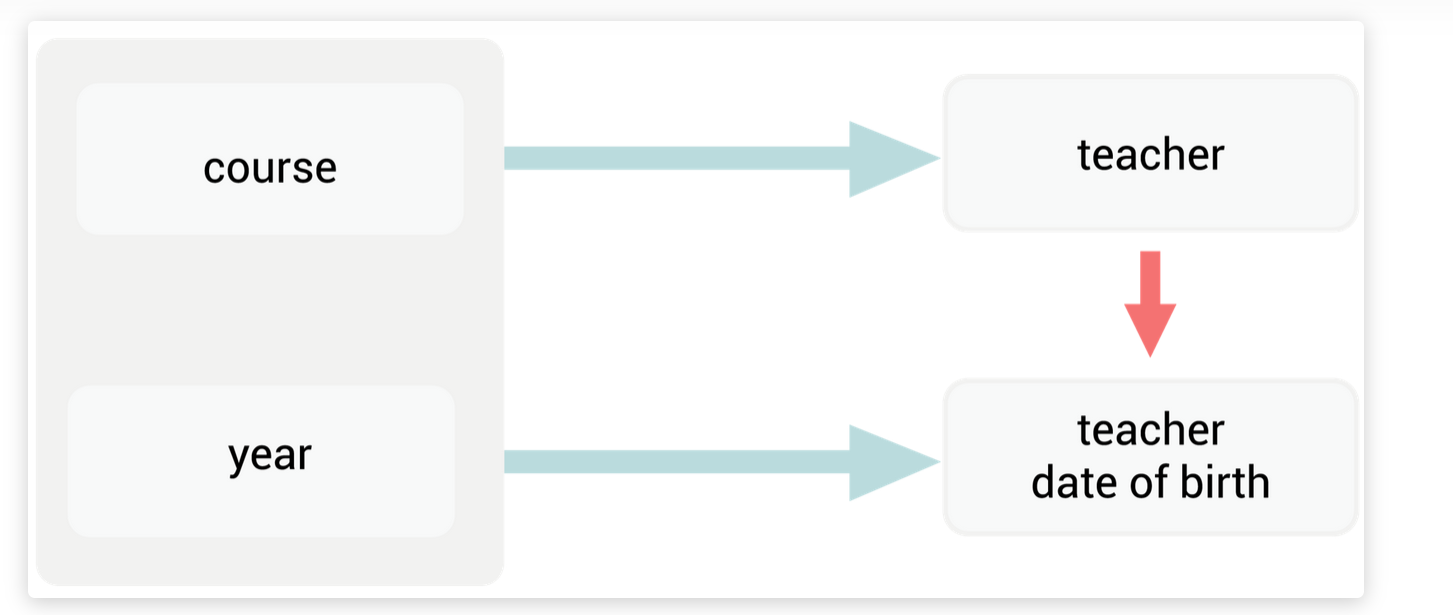
\includegraphics[width=0.5\textwidth]{assets/third_normal_form.png}
    \caption{Third Normal Form}
\end{figure}

\textbf{Higher Form - Decomposition Algorithm}
\begin{enumerate}
    \item Identify the dependencies that violate the BCNF definition and consider that as
          $X \rightarrow A$.
    \item Decompose the relation $R$ into $XA$ and $R - \{A\}$ ($R$ minus $A$).
    \item Validate if both the decompositions are in BCNF or not. If not, re-apply the
          algorithm on the decomposition that is not in BCNF.
\end{enumerate}

\begin{figure}[h]
    \centering
    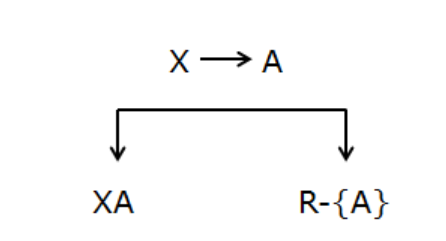
\includegraphics[width=0.7\textwidth]{assets/BCNF_decomposition.png}
    \caption{BCNF Decomposition}
\end{figure}

\begin{align*}
    R1 &= \{A, B, C, D, E\} \\
    AB &\rightarrow CD \\
    D &\rightarrow E \\
    A &\rightarrow C \\
    B &\rightarrow D \\
\end{align*}

Candidate Key:$ AB$

Prime Attributes: $A, B$

Non-Prime Attributes: $C, D, E$

\begin{align*}
    AB &\rightarrow CD \ (\text{Full Dependency - CD is dependent on the candidate key}) \\
    D &\rightarrow E \ (\text{Transitive Dependency: non-prime derives non-prime}) \\
    A &\rightarrow C \ (\text{Partial Dependency: Prime derives non-prime}) \\
    B &\rightarrow D \ (\text{Partial Dependency: Prime derives non-prime}) \\
\end{align*}
Hence the dependencies that violate BCNF are D -> E, A -> C, B -> D.
So, we will take $D \rightarrow E$ first as $X \rightarrow A$ (not the A listed in relation as attributes). So $X = D$ and $A = E$. $XA$ will be $DE$ and $R - \{A\}$ will be $ABCD$.
\begin{figure}[h]
    \centering
    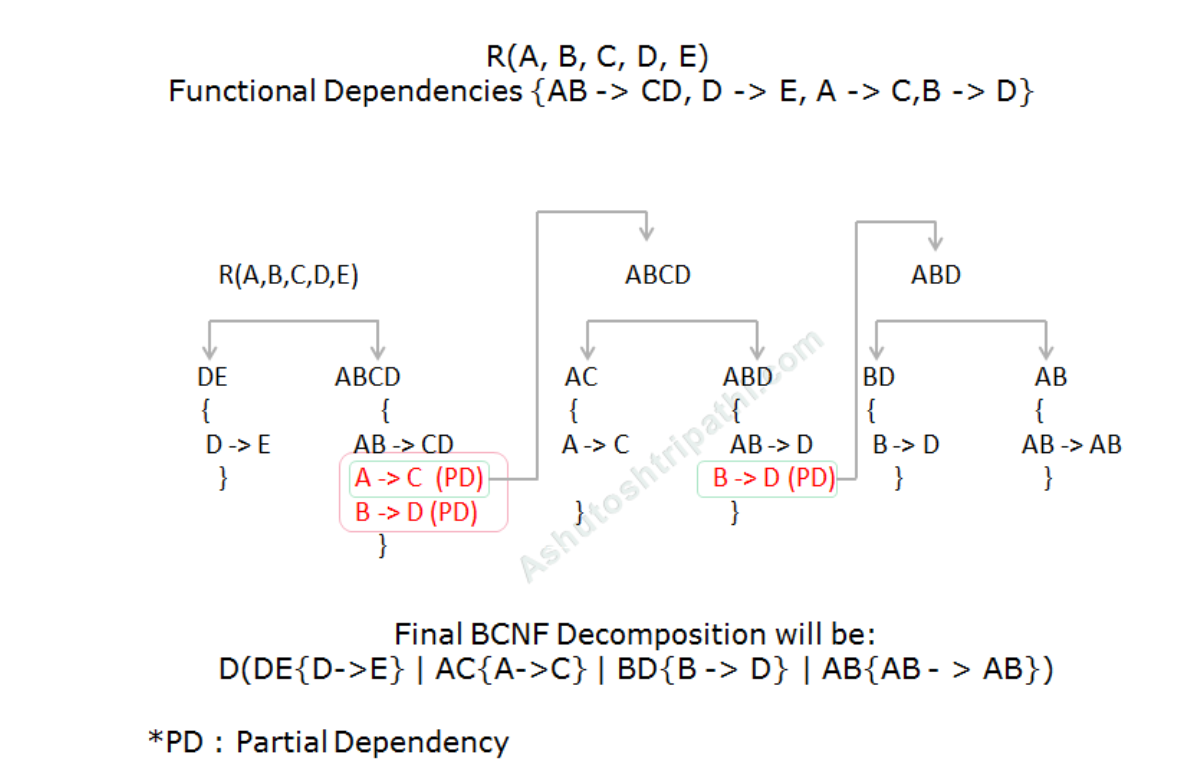
\includegraphics[width=0.5\textwidth]{assets/BCNF.png}
    \caption{BCNF}
\end{figure}

\subsection{Boyce-Codd Normal Form}
\begin{itemize}
    \item Each attribute in the table must depend on the key, the whole key, and nothing
          but the key.
    \item If everything on the right is a full key, it is fine (but check again).
\end{itemize}
\textbf{Nothing but the Key}
\begin{itemize}
    \item All arrows must be out of candidate keys.
    \item Check if you have a super key with transitivity for each key.
\end{itemize}

\begin{figure}[h]
    \centering
    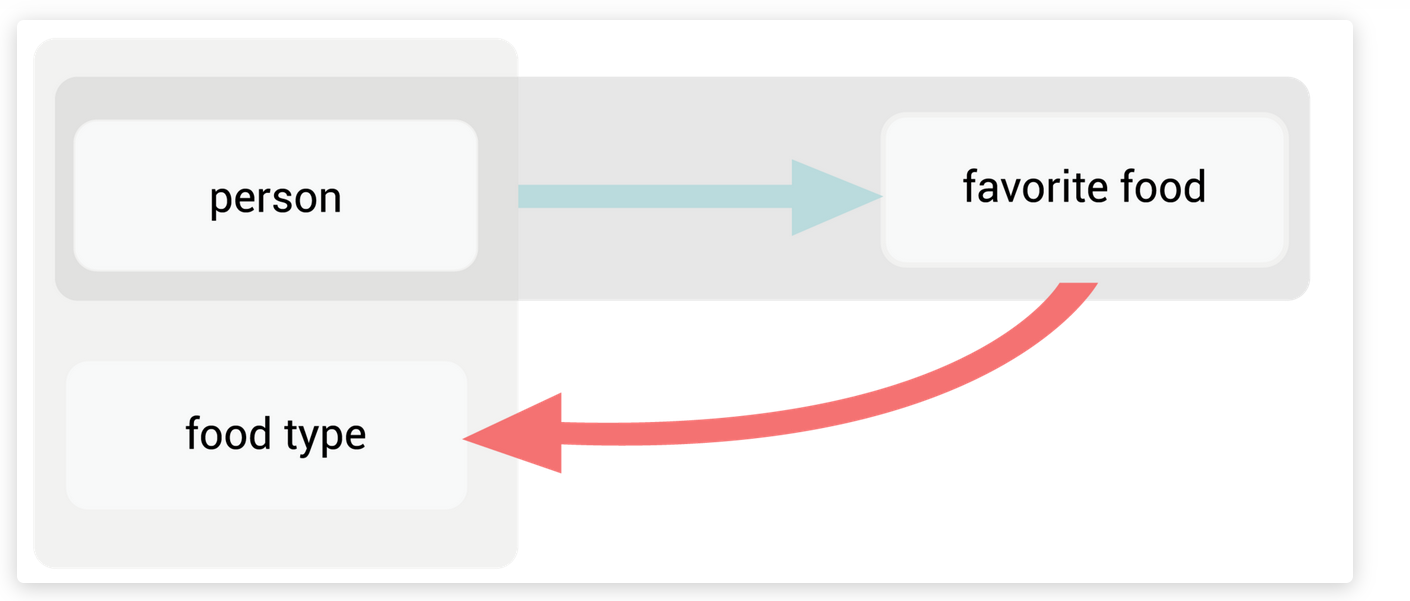
\includegraphics[width=0.5\textwidth]{assets/b_normal_form.png}
    \caption{Boyce-Codd Normal Form}
\end{figure}

\subsection{Fourth Normal Form}
The only kinds of multivalued dependency allowed in a table are multivalued
dependencies on the key.

\subsection{Fifth Normal Form}
It must not be possible to describe the table as being the logical result of
joining some other tables together.

\section{Candidate Key}
\begin{itemize}
    \item You have a candidate key if all its attributes appear only on the left side of
          the dependencies.
    \item To get the candidate key, look at the closure. If you can reach all the
          important values, it is a super key for sure. If it is the only one, then it is
          even a candidate key.
\end{itemize}

\section{Minimal Basis}
\begin{align*}
    A &\rightarrow BC \\
    B &\rightarrow C \\
    A &\rightarrow B \\
    AB &\rightarrow C \\
\end{align*}

\begin{enumerate}
    \item Convert right-hand-side attributes into singleton attributes
    \begin{align*}
        A &\rightarrow B \\
        A &\rightarrow C \\
        B &\rightarrow C \\
        A &\rightarrow B \\
        AB &\rightarrow C \\
    \end{align*}
    
    \item Remove the extra left-hand-side attribute

          Find the closure of A

          $A^+ = \{A, B, C\}$

          So, $AB \rightarrow C$ can be converted into $A \rightarrow C$
          \begin{align*}
              A & \rightarrow B \\
              A & \rightarrow C \\
              B & \rightarrow C \\
              A & \rightarrow B \\
              A & \rightarrow C
          \end{align*}

          Remove redundant functional dependencies

          \begin{align*}
              A & \rightarrow B \\
              B & \rightarrow C
          \end{align*}

          Now, we will convert the above set of FDs into the canonical cover.

          The canonical cover for the above set of FDs will be as follows:
          \begin{align*}
              A & \rightarrow BC \\
              B & \rightarrow C
          \end{align*}
\end{enumerate}

\section{Example}
To get the minimal cover, you have to make two steps. To demonstrate, I'll
first split the dependencies into multiple (only one attribute on the right
side) to make it more clean:
\begin{align*}
    A    & \rightarrow B \\
    ABCD & \rightarrow E \\
    EF   & \rightarrow G \\
    EF   & \rightarrow H \\
    ACDF & \rightarrow E \\
    ACDF & \rightarrow G \\
\end{align*}
The following steps must be done in this order (\#1 and then \#2), otherwise
you can get an incorrect result. \textbf{Step 1: Get rid of redundant
    attributes (reduce left sides):} Take each left side and try to remove one each
attribute one at a time, then try to deduce the right side (which is now only
one attribute for all dependencies). If you succeed, you can then remove that
letter from the left side, then continue. Note that there might be more than
one correct result; it depends on the order in which you do the reduction. You
will find out that you can remove B from the dependency $ABCD \rightarrow E$
because $ACD \rightarrow ABCD$ (use the first dep.) and from $ABCD \rightarrow
    E$. You can use the full dep. you are currently reducing; this is sometimes
confusing at first, but if you think about it, it will become clear that you
can do that. Similarly, you can remove F from $ACDF \rightarrow E$ because $ACD
    \rightarrow ABCD \rightarrow ABCDE \rightarrow E$ (you can obviously deduce a
single letter from the letter itself). After this step, you get:
\begin{align*}
    A   & \rightarrow  B \\
    ACD & \rightarrow  E \\
    EF  & \rightarrow  G \\
    EF  & \rightarrow  H \\
    ACD & \rightarrow  E \\
    ACD & \rightarrow  G \\
\end{align*}
These rules still represent the same dependencies as the original. Note that now we have a duplicate rule $ACD \rightarrow E$. If you look at the whole thing as a set (in the mathematical sense), then of course, you can't have the same element twice in one set. For now, I'm just leaving it twice here because the next step will get rid of it anyway.
\textbf{Step 2: Get rid of redundant dependencies}
Now for each rule, try to remove it and see if you deduce the same rule by only using others. In this step, you, of course, cannot use the dep. you're currently trying to remove (you could in the previous step).
If you take the left side of the first rule $A \rightarrow B$, hide it for now, you see you can't deduce anything from $A$ alone. Therefore, this rule is not redundant. Do the same for all others. You'll find out that you can (obviously) remove one of the duplicate rules $ACD \rightarrow E$, but strictly speaking, you can use the algorithm also. Hide only one of the two same rules, then take the left side $(ACD)$, and use the other to deduce the right side. Therefore, you can remove $ACD \rightarrow E$ (only once, of course).
You'll also see you can remove $ACDF \rightarrow G$, because $ACDF \rightarrow ACDFE \rightarrow G$. Now the result is:
\begin{align*}
    A   & \rightarrow B \\
    EF  & \rightarrow G \\
    EF  & \rightarrow H \\
    ACD & \rightarrow E \\
\end{align*}
Which is the minimal cover of the original set.
\section{SQL Difference On, Where}
The information is from \cite{sql-stackoverflow}.
\begin{itemize}
    \item Does not matter for inner joins
    \item Matters for outer joins
\end{itemize}
a. \texttt{WHERE} clause: After joining. Records will be filtered after the join has taken place.
b. \texttt{ON} clause - Before joining. Records (from the right table) will be filtered before joining. This may end up as null in the result (since OUTER join).
\section{SQL \texttt{WITH}}
\begin{itemize}
    \item Referencing a temporary table multiple times in a single query
    \item Performing multi-level aggregations, such as finding the average of maximums
    \item Performing an identical calculation multiple times over within the context of a
          larger query
    \item Using it as an alternative to creating a view in the database
\end{itemize}

\begin{table}[h]
    \centering
    \begin{tabular}{|c|c|c|c|}
        \hline
        OrderDetailID & OrderID & ProductID & Quantity \\
        \hline
        1             & 10248   & 11        & 12       \\
        2             & 10248   & 42        & 10       \\
        3             & 10248   & 72        & 5        \\
        4             & 10249   & 14        & 9        \\
        5             & 10249   & 51        & 40       \\
        \hline
    \end{tabular}
    \caption{Sample OrderDetails Table}
\end{table}

The objective is to return the average quantity ordered per ProductID:

\begin{align*}
    \text{WITH cte\_quantity} & \text{ AS}                                   \\
                              & \text{SELECT}                                \\
                              & \text{SUM(Quantity) as Total}                \\
                              & \text{FROM OrderDetails}                     \\
                              & \text{GROUP BY ProductID}                    \\
                              &                                              \\
    \text{SELECT}                                                            \\
                              & \text{AVG(Total) average\_product\_quantity} \\
                              & \text{FROM cte\_quantity;}
\end{align*}

\section{SQL \texttt{OVER}}

\begin{table}[h]
    \centering
    \begin{tabular}{|c|c|c|c|c|c|c|}
        \hline
        sale\_day  & sale\_month & sale\_time & branch   & article    & quantity & revenue \\
        \hline
        2021-08-11 & AUG         & 11:00      & New York & Rolex P1   & 1        & 3000.00 \\
        2021-08-14 & AUG         & 11:20      & New York & Rolex P1   & 2        & 6000.00 \\
        2021-08-17 & AUG         & 10:00      & Paris    & Omega 100  & 3        & 4000.00 \\
        2021-08-19 & AUG         & 10:00      & London   & Omega 100  & 1        & 1300.00 \\
        2021-07-17 & JUL         & 09:30      & Paris    & Cartier A1 & 1        & 2000.00 \\
        2021-07-11 & JUL         & 10:10      & New York & Cartier A1 & 1        & 2000.00 \\
        2021-07-10 & JUL         & 11:40      & London   & Omega 100  & 2        & 2600.00 \\
        2021-07-15 & JUL         & 10:30      & London   & Omega 100  & 3        & 4000.00 \\
        \hline
    \end{tabular}
    \caption{Sample Sales Table}
\end{table}

The window frame is a set of rows that depends on the current row; thus, the
set of rows could change for each row processed by the query. We define window
frames using the \texttt{OVER} clause. The syntax is:
\[
    \text{OVER ([PARTITION BY columns] [ORDER BY columns])}
\]
The \texttt{PARTITION BY} subclause defines the criteria that the records must
satisfy to be part of the window frame. In other words, \texttt{PARTITION BY}
defines the groups into which the rows are divided; this will be clearer in our
next example query. Finally, the \texttt{ORDER BY} clause defines the order of
the records in the window frame.
Let’s see the SQL \texttt{OVER} clause in action. Here’s a simple query that
returns the total quantity of units sold for each article.
\[
    \text{SELECT sale\_day, sale\_time,} \\
    \text{branch, article, quantity, revenue,} \\
    \text{SUM(quantity) OVER (PARTITION BY article) AS total\_units\_sold} \\
    \text{FROM sales}
\]
This query will show all the records of the \texttt{sales} table with a new
column displaying the total number of units sold for the relevant article. We
can obtain the quantity of units sold using the \texttt{SUM} aggregation
function, but then we couldn’t show the individual records.
In this query, the \texttt{OVER PARTITION BY} article subclause indicates that
the window frame is determined by the values in the article column; all records
with the same article value will be in one group.
\section{View}

An \texttt{UPDATE} statement against a View can only affect one target table at
a time, and your \texttt{UPDATE} statement cannot update data in a derived
column.

\section{Referential Constraints}

\subsection{Cascade}

\begin{itemize}
    \item Propagate update or delete
\end{itemize}

\subsection{Restrict}

\begin{itemize}
    \item Prevent deletion of the primary key before trying to do the change, cause an
          error
    \item Throw error immediately
\end{itemize}

\subsection{No Action}

\begin{itemize}
    \item Prevent modifications after attempting the change cause an error
    \item Throw error after trying
\end{itemize}

\subsection{Set Default, Set Null}

\begin{itemize}
    \item Set referenced to NULL or to a default value
\end{itemize}

\section{Keys}

\subsection{Super Key}

\begin{itemize}
    \item Like a superset
    \item Uniquely identify the tuple
    \item ID, Name; ID, Phone; Name, Phone, etc.
    \item May contain extraneous attributes
\end{itemize}

\subsection{Candidate Key}

\begin{itemize}
    \item Minimal super keys are called candidate keys
\end{itemize}

\subsection{Primary Key}

\begin{itemize}
    \item Unique
    \item Should not have null values (email, phone number is not that good)
\end{itemize}

\section{Database Systems}

\subsection{Disk Manager}

\begin{itemize}
    \item Allocates, deletes, fetches pages
    \item No other layer has to interact with the disk directly
\end{itemize}

\subsection{Buffer Pool Manager}

\begin{itemize}
    \item Maintains an in-memory buffer
    \item Upper layers have the illusion that the entire data is in memory and not on
          disk
    \item Provides functionality to fetch and update pages
\end{itemize}

\subsection{Access Methods}

\begin{itemize}
    \item Sequential Scan
    \item B-Tree Index
    \item Hash Table
    \item Sort
\end{itemize}
It provides a higher-level abstraction to access information in a table without
interacting with the buffer or disk.

\subsection{Operator Execution}

Executes a relational algebra:

\begin{itemize}
    \item Join
    \item Projection
    \item Select
\end{itemize}

\subsection{Query Optimization}

Generates a good execution plan.

\subsection{Heap File}

A heap file is an unordered collection of pages where tuples are stored in
random order.

\subsection{Record ID}

\((Page ID, Slot ID)\)

\subsection{Pages}

A page is a fixed-size block of data:

\begin{itemize}
    \item Contain tuples, metadata, indexes, log records, etc.
\end{itemize}

\subsection{Different Joins}

\subsubsection{Sort Merge Join (equi-join)}

\begin{itemize}
    \item Efficient: Sorted attribute (e.g., clustered index)
    \item Inefficient: Unsorted attribute
\end{itemize}

\subsubsection{Nested Loop Join}

\begin{itemize}
    \item Efficient: Smaller relation fits into memory
    \item Inefficient: Both relations do not fit into memory
    \item \(B(R) + |R| \cdot B(S)\)
\end{itemize}

\subsubsection{Block Nested Loop Join (equi-join)}

\subsubsection{Index Nested Loop Join (equi-join)}

\begin{itemize}
    \item Efficient: Low selectivity (few reads per disk)
    \item Inefficient: High selectivity (loads of reads per disk)
\end{itemize}

\subsubsection{Hash Join (equi-join)}

\begin{itemize}
    \item If the Hash table fits in DRAM: \(B(S) + B(R)\)
    \item Very efficient
    \item Hash join algorithms are in general only applicable to equi joins and natural
          joins
    \item Efficient: Result of join fits into memory
    \item Inefficient: Result doesn't fit into memory
    \item Solution: Grace Hash Join
\end{itemize}

\subsubsection{Grace Hash Join}

\(3(B(R) + B(S))\)
All data ends up in the same partition or all data ends up in the same hash bucket, then the Grace Hash algorithm performs worse \cite{database-lecture}.

\subsection{Lossless}

\begin{align*}
    S & = S_1 \cup S_2    \\
    S & = S_1 \bowtie S_2
\end{align*}

\subsection{Quiz Questions and Answers}

\subsubsection{While adding tuples to a page, both the slot array and the data of the tuples will grow from the beginning to the end:}

The slot array will grow from the beginning to the end, whereas the data of the
tuples will grow from the end to the beginning. When they meet, the page
becomes full \cite{database-lecture}.

\subsubsection{Sequential Scan or B-Tree}

When nearly all the tuples fulfill the requirement, scan is fast, B - Tree is
slow. When only a few or only one fulfills the requirement, B - Tree is fast,
scan is slow.

\[
    T_{\text{scan}} = T_{\text{access}} + \frac{\text{(pageSize *  m)}}{\text{Bandwidth}}
\]

\[
    T_{\text{index}}(k) = (T_{\text{access}} \frac{\text{page size}}{\ldots})
\]

\section{Recoverability}

\subsection{Recoverable (RC)}

If \(T_i\) reads from \(T_j\) then \(c_j < c_i\). Each transaction commits only
after each transaction from which it has read has committed. No need to undo a
committed transaction.

\begin{figure}[h]
    \centering
    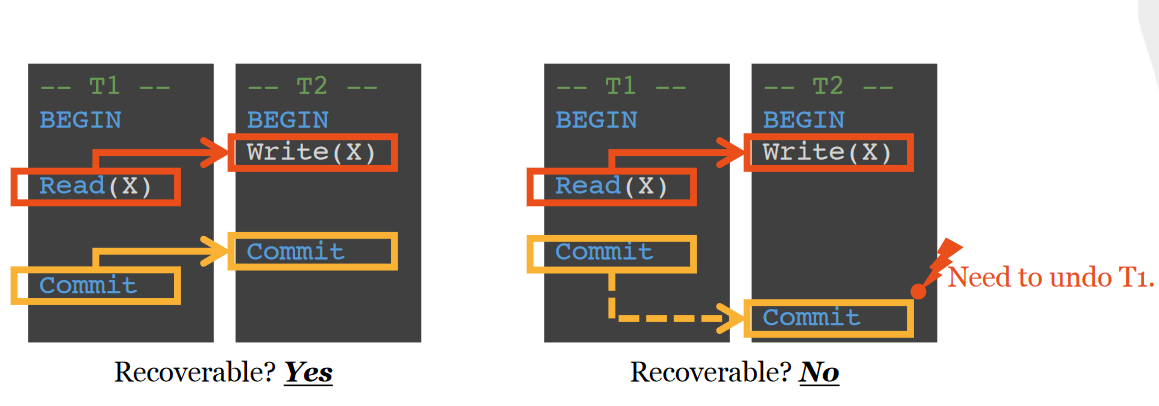
\includegraphics[width=0.8\textwidth]{assets/recoverable.png}
    \caption{Recoverable Schedule \cite{database-lecture}}
\end{figure}

\subsection{Avoids Cascading Aborts (ACA)}

If \(T_i\) reads \(X\) from \(T_j\) and commits then \(c_j < r_i[x]\).
\(r_i[X]\) is the time \(T_i\) reads \(X\). Avoids cascading rollback if
transactions may read only values written by committed transactions. Aborting a
transaction does not cause aborting others.

\begin{figure}[h]
    \centering
    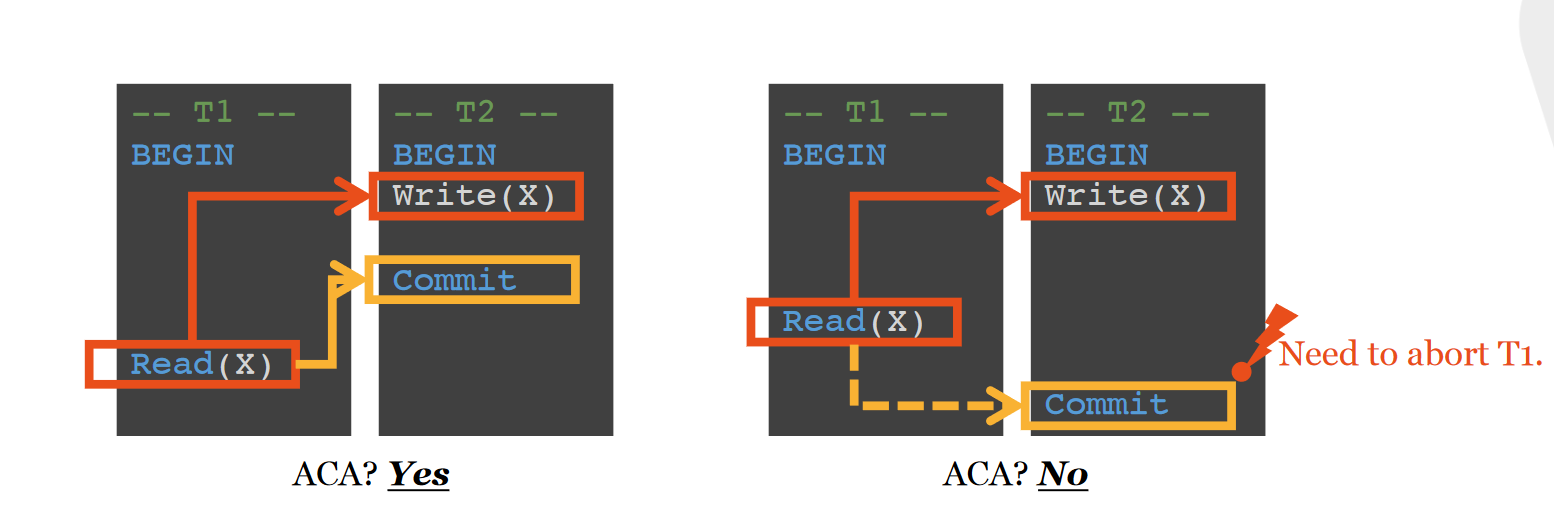
\includegraphics[width=0.8\textwidth]{assets/aca.png}
    \caption{Avoids Cascading Aborts Schedule \cite{database-lecture}}
\end{figure}

\section*{Strict (ST)}
\begin{itemize}
    \item If $T_i$ reads from or overwrites a value written by $T_j$, then $(c_j <
              r_i[X]$ AND $c_j < w_i[X])$ or $(a_j < r_i[X]$ AND $a_j < w_i[X])$
    \item $a_j$ is the abort time of $T_j$
    \item Transaction must not release any exclusive locks until the transaction has
          either committed or aborted, and the commit or abort log record has been
          flushed to disk.
          \begin{itemize}
              \item A schedule of transactions that follow the strict-locking rule is called a
                    strict schedule.
              \item Undoing a transaction does not undo the changes of other transactions.
          \end{itemize}
\end{itemize}

\begin{figure}[h]
    \centering
    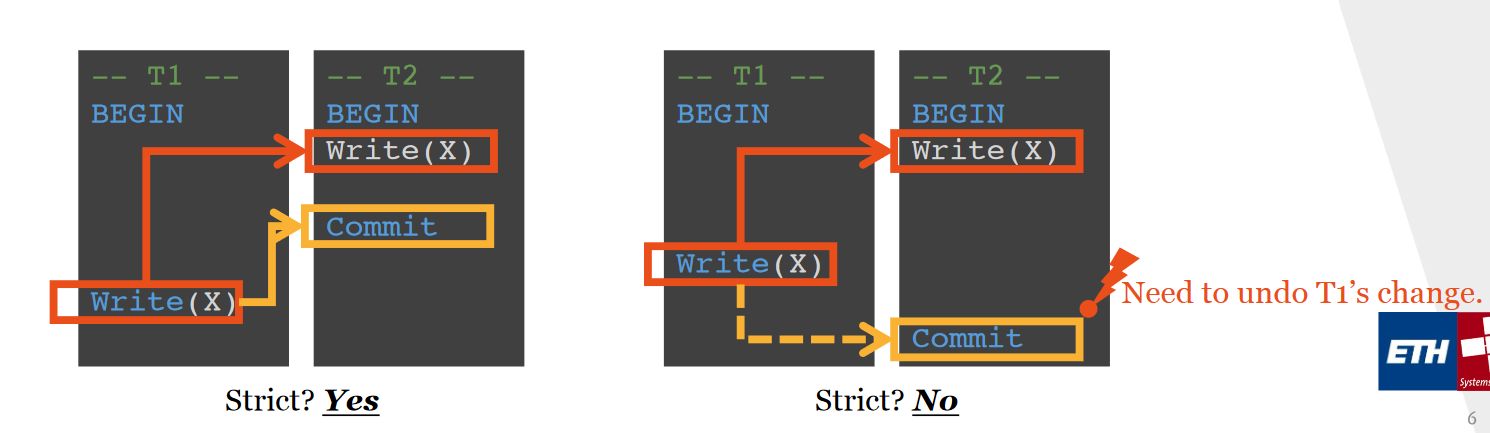
\includegraphics[width=0.5\textwidth]{assets/strict.png}
    \caption{Strict Schedule Diagram}
\end{figure}

\section*{Serializable}
Defined by the equivalence of result.

\section*{Conflict Serializable}
Defined by swap adjacent, non-conflicting, operations. Conflict Serializable is a \textbf{subset} of Serializable.

\section*{How to decide Conflict-Serializability?}
\begin{itemize}
    \item Go from definition -- do the swap.
    \item Dependency Graph.
          \begin{itemize}
              \item You can ignore the aborts.
              \item No reads, then it is automatically recoverable and ACA $\rightarrow$ just need
                    to check strict.
          \end{itemize}
\end{itemize}

\section*{Snapshot Isolation}
\begin{itemize}
    \item When a transaction $T$ starts, it receives a timestamp $TS(T)$.
    \item All reads are carried out as of the DB version of $TS(T)$.
    \item All writes are carried out in a separate buffer.
    \item When a transaction commits, DBMS checks for conflicts - Abort $T_1$ if there
          exists $T_2$ such that $T_2$ committed after $TS(T_1)$ and before $T_1$
          commits, and $T_1$ and $T_2$ updated the same object.
    \item Writes and readers do not block each other.
    \item Concurrency and availability.
          \begin{itemize}
              \item No read or write of a transaction is ever blocked.
          \end{itemize}
    \item Overhead.
          \begin{itemize}
              \item Need to keep the write-set of a transaction only.
              \item Very efficient way to implement aborts.
          \end{itemize}
    \item No deadlocks, but unnecessary rollbacks.
\end{itemize}

\begin{figure}[h]
    \centering
    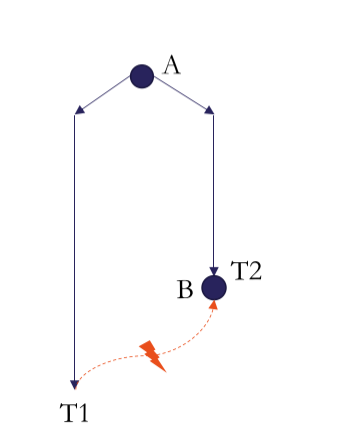
\includegraphics[width=0.7\textwidth]{assets/snapshot_isolation.png}
    \caption{Snapshot Isolation Diagram}
\end{figure}

\section*{Two Phase Locking}
\textbf{Phase 1: Growing}
\begin{itemize}
    \item Each transaction requests the lock that it needs from the DBMS's lock manager.
    \item It cannot release locks in phase 1.
\end{itemize}

\textbf{Phase 2: Shrinking}
\begin{itemize}
    \item Transaction is only allowed to release locks that it previously required. It
          cannot acquire new locks.
    \item Guarantees conflict serializability.
          \begin{itemize}
              \item Only generates schedules whose dependency graph is acyclic.
          \end{itemize}
\end{itemize}

\begin{figure}[h]
    \centering
    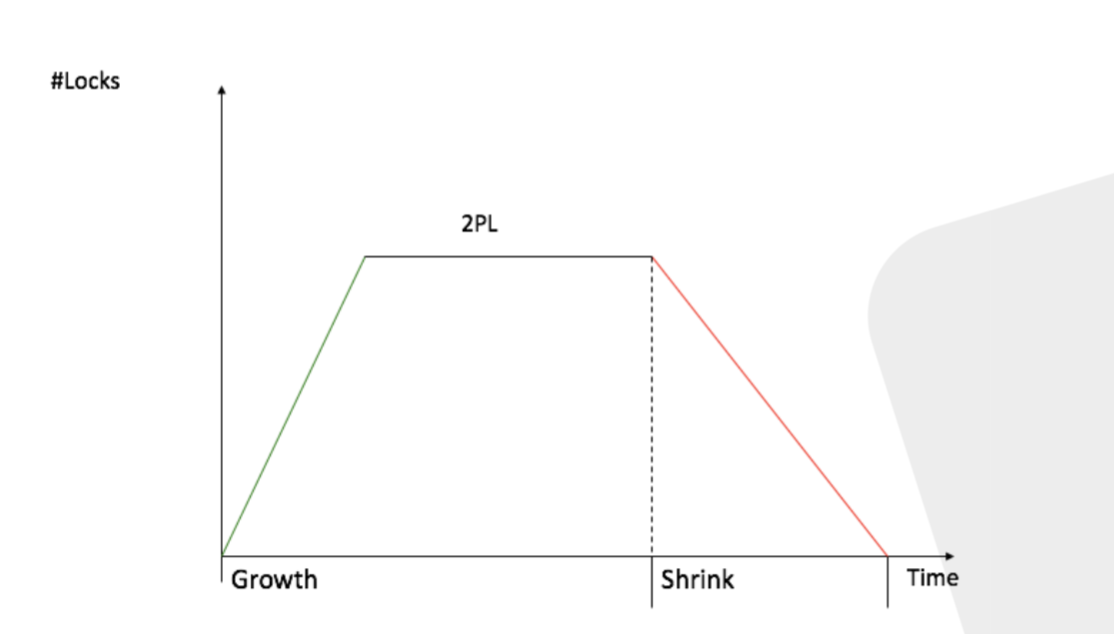
\includegraphics[width=0.7\textwidth]{assets/two_phase_locking.png}
    \caption{Two Phase Locking Diagram}
\end{figure}

\section*{Strict Two Phase Locking}
At phase 2: all locks are kept until the end of the transaction (commit or abort).

\begin{figure}[h]
    \centering
    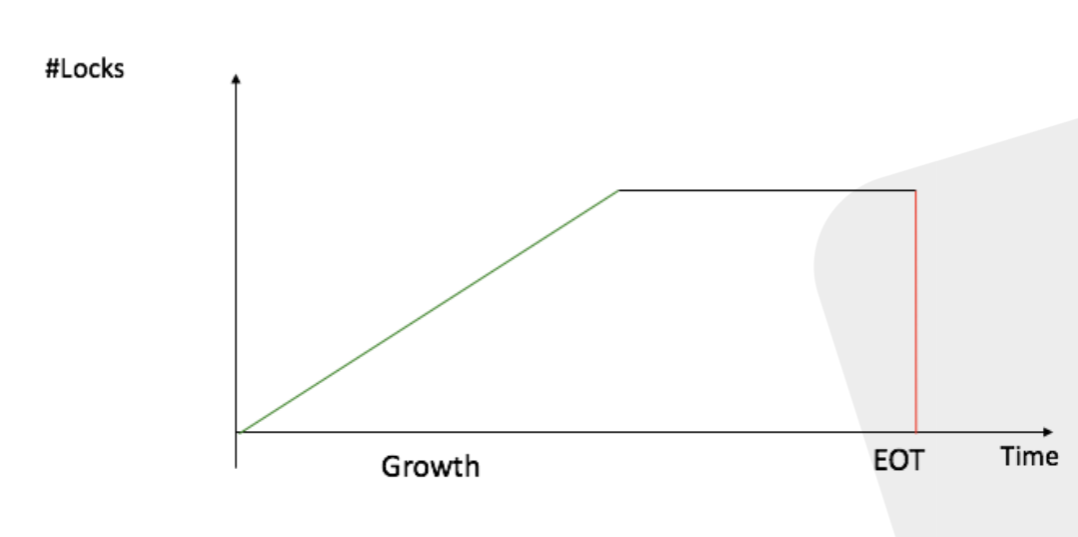
\includegraphics[width=0.5\textwidth]{assets/strict_two_phase_locking.png}
    \caption{Strict Two Phase Locking Diagram}
\end{figure}

\end{document}
